%!TEX root = 00_main.tex

\begin{figure*}
    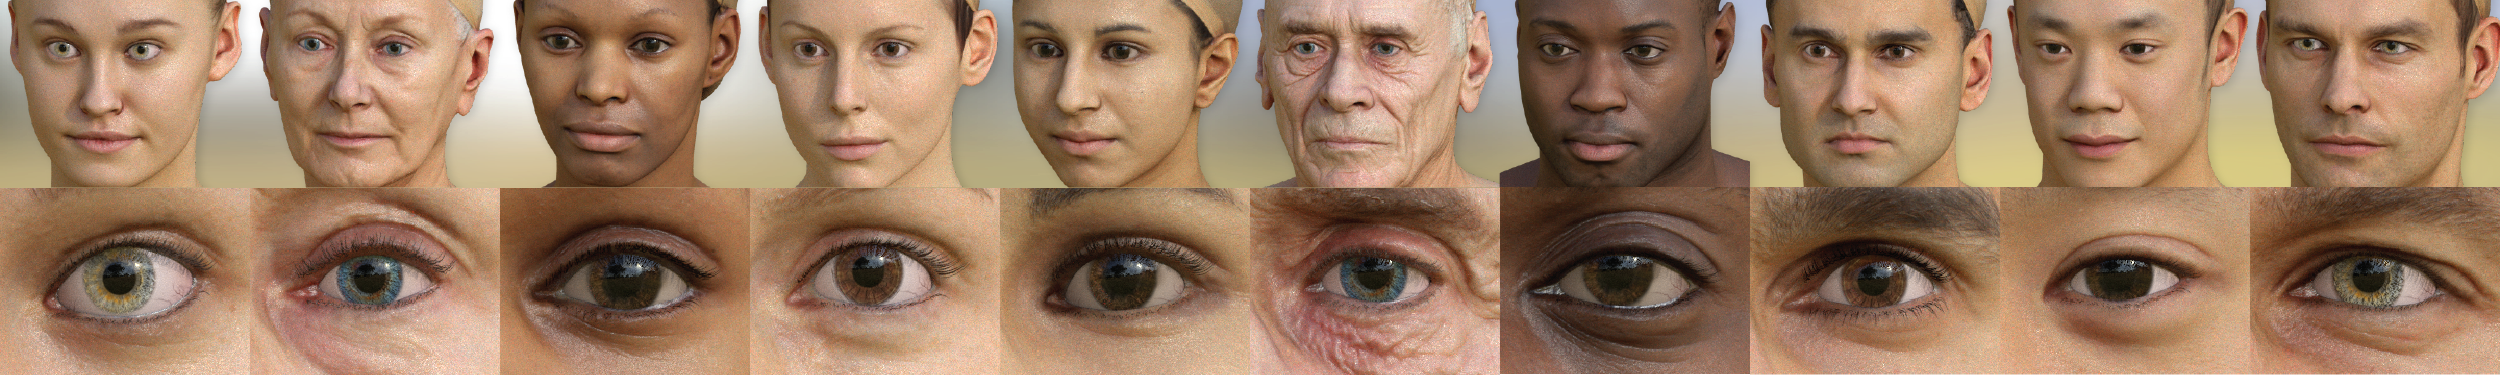
\includegraphics[width=\textwidth]{model_suite}
    \caption{Set of head models and corresponding close-ups of the eye regions used in our method. The set includes 10 different head models of both genders that cover a range of ethnicities and ages.}
    \label{fig:model_suite}
\end{figure*}

\section{Dynamic Eye-Region Model}

We developed a realistic dynamic eye-region model which can be randomly posed to generate fully labeled training images.
\autoref{fig:process} provides an overview of the model preparation process.
% For a set of training images to be useful, it should be large, representitive of real-world variety, and cleanly labelled.
For the resulting training data to be useful, it should be representative of real-world variety.
Our goal therefore was to model the continuous changes in appearance that the face and eyes undergo during eye movement, so they are accurately represented in close-up synthetic eye images.
This is more challenging than simply rendering a collection of static models, as dynamic geometry must be correctly topologized and rigged to be able to deform continuously.
To achieve this, we combine scanned facial geometry with a separate controllable eye model. These can together be posed to synthesize labelled training data.
% Appearance-wise, the eye-region is one of the most complex areas of the whole body -- separate parts can all move independently, and feature a range of reflectance properties and small-scale details.
% The eyelids, upper-cheek, and eye-ball can all move independently, and feature a range of reflectance properties and small-scale details.
%
In this section we first present our anatomically inspired computer graphics eyeball model, and then explain our procedure for converting a collection of static 3D head scans into dynamic eye-region models that can assume a range of realistic poses.
%\commentA{I think it would be good to first describe in 1-2 paragraphs what the particular challenges of modelling eye shape, dynamics etc. are. This gives better context for the method description that follows and hopefully also underlines that this is a non-trivial task and the work therefore a significant step forward.}

%\todo{past tense}
%\commentA{we have to explain what makes the model dynamic}
%\commentA{could be nice to show existing renderings and ours side by side, e.g. Leszeks and others (if any)}

\subsection{Simplified Eyeball Model}
\label{subsec:eyeball_model}

\begin{figure}
    \captionsetup[subfigure]{labelformat=empty} % stop subcaption writing "(a)""
    \captionsetup{subrefformat=parens} % add parentheses to \subref
    \begin{subfigure}[t]{0.33\columnwidth}
        \inlinelabel{a}{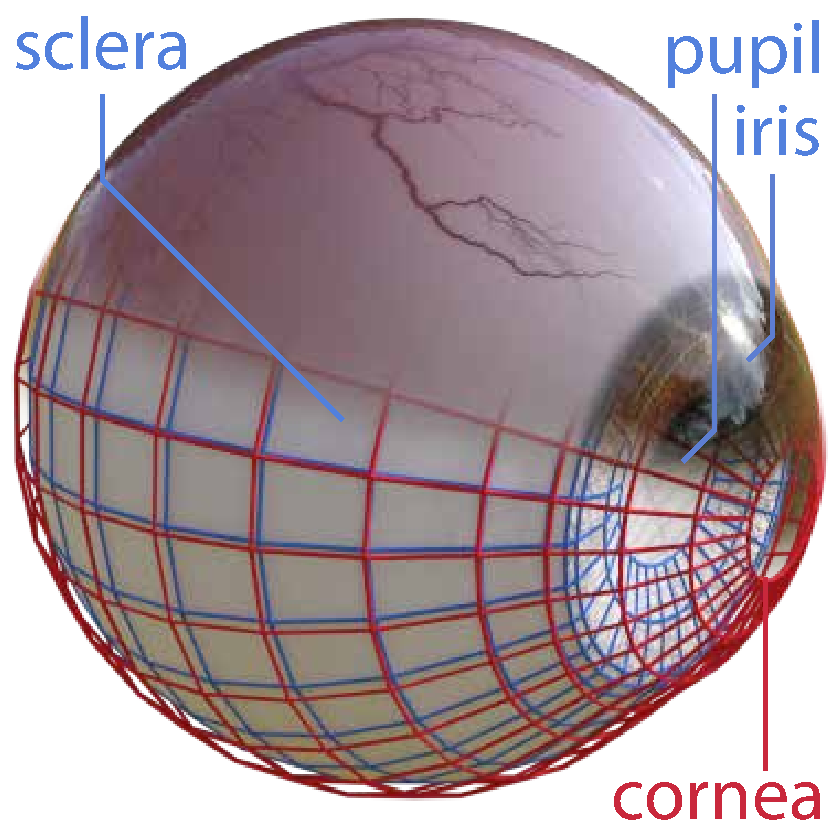
\includegraphics[width=\textwidth]{eye_model}}
        \caption{}\label{fig:eye_model_parts}
    \end{subfigure}
    \hfill
    \begin{subfigure}[t]{0.65\columnwidth}
        \inlinelabel{b}{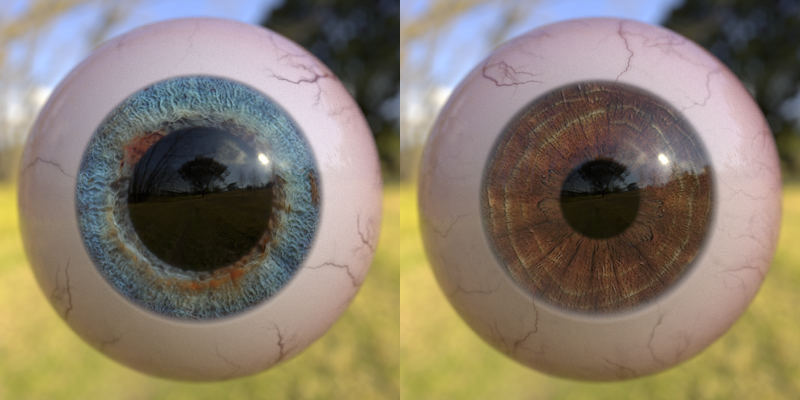
\includegraphics[width=\textwidth]{eye_examples}}
        \caption{}\label{fig:eye_model_images}
    \end{subfigure}
    \par\vspace{-28pt}
    \caption{Our eye model includes the sclera, pupil, iris, and cornea \subref{fig:eye_model_parts} and can exhibit realistic variation in both shape (pupillary dilation) and texture (iris color, scleral veins) \subref{fig:eye_model_images}.}
    \label{fig:eye_model}
\end{figure}

% It is important to accurately model reflections and refractions in the eye as they can lead to specular highlights -- these common eye-region image features are often used by eye-tracking algorithms, or can confound approaches that are not robust.

Our eye model consists of two parts (see~\autoref{fig:eye_model_parts}).
The outer part (red wireframe) approximates the eye's overall shape with two spheres ($r_1\!=\!12\textrm{mm}, r_2\!=\!8\textrm{mm}$ \cite{ruhland2014look}), the latter representing the corneal bulge.
To avoid a discontinuous seam between spheres, their meshes were joined, and the vertices along the seam were smoothed to minimize differences in face-angle.
% \commentA{how joined and smoothed?} Erroll - Maybe needs rewording. Perhaps i'll just put a citation for the smoothing operation? I don't particularly want to describe it
This outer part is transparent, refractive ($n\!=\!1.376$), and partially reflective.
The sclera's bumpy surface is modelled with smoothed solid noise functions, and applied using a \emph{displacement map} -- a 2D scalar function that shifts a surface in the direction of its normal \cite{lee2000displaced}.
The inner part (blue wireframe) is a flattened sphere  -- the planar end represents the iris and pupil, and the rest represents the sclera, the white of the eye.
There is a $0.5\textrm{mm}$ gap between the two parts which accounts for the thickness of the cornea.
% \commentE{compare with recent Disney work}

Eyes exhibit variation in both shape (pupillary dilation) and texture (iris color and scleral veins).
To model shape variation we use \emph{blend shapes} -- an animation technique where several different poses are created for the same topological mesh, and then interpolated between \cite{orvalho2012facial}. 
We created blend shapes for dilated and constricted pupils, as well as large and small irises to account for a small amount ($10\%$) of variation in iris size.
% Maybe try to explain blend shapes better
% Blend shapes are localized so can be mixed, so we can easily model an eye with a small pupil, and a large iris.
We vary the texture of the eye by randomly compositing images in three separate layers:
\begin{inparaenum}[\itshape i\upshape)]
\item a \emph{sclera} tint layer (white, pink, or yellow);
\item an \emph{iris} layer with four different photo-textures (amber, blue, brown, grey); and
\item a \emph{veins} layer (blood-shot or clear).
\end{inparaenum}
% We matched the sclera tint to each separate face model but uniformably randomly varied iris color.
% Maybe move to related work?
% Previous research on iris-synthesis \commentE{cite} would have allowed continually different iris textures, but we decided this added complexity would not make a worthwhile improvement in overall appearance variation, especially when rendered at lower resolutions.

\subsection{3D Head Scan Acquisition}
\label{sec:eye_region_geom_prep}

For an eye-region rendering to be realistic, it must also feature realistic nearby face detail.
While previous approaches used lifelike artist-created models, for example~\cite{swirski2014rendering}, we instead rely on high-quality head scans captured by a professional photogrammetry studio (10K diffuse color textures, 0.1mm resolution geometry)\footnote{Ten24 3D Scan Store -- \url{http://www.3dscanstore.com/}}.
%\cite{Ten24}.
%\commentA{link or even better reference if available}
%Nowadays it is possible to purchase such scans online (from $\sim\!\$15$/scan)
%or use free or commercial photogrammetry software to generate facial geometry models in-house.
Facial appearance around the eye varies dramatically between people as a result of different eye-shapes (e.g. round vs hooded), orbital bone structure (e.g. deep-set vs protruding), and skin detail (wrinkled vs smooth). Therefore our head models (see \autoref{fig:model_suite}) cover both genders with a variety of ethnicities and ages.

\subsection{Eye-Region Geometry Preparation}

As can be seen in \autoref{fig:process_original_scan}, the cornea of the original head scan has been incorrectly reconstructed by the optical scanning process.
This is because transparent surfaces are not directly visible, so cannot be reconstructed in the same way as diffuse surfaces, such as skin.
% Recent work used a hybrid reconstruction method to reconstruct the corneal surface separately, but requires additional hardware \cite{berard2014highquality} -- this level of detail was deemed unnecessary for our purposes.
We wanted images representing a wide range of eye-gaze directions, so we needed to be able to pose the eyeball separately from the face geometry.
We therefore removed the scanned eyeball from the mesh, and placed our own eyeball approximation in its place.
% \commentY{I feel this part should be explained beforehand,  i.e., we should first explain why take this approach combining eye model and face scan}

While the original head scan geometry is suitable for being rendered as a static model, its high resolution topology cannot be easily controlled changes in eye-region shape.
\commentA{the following reference is not strictly needed and could be removed to make space for affective computing reference}
Vertical saccades are always accompanied by eyelid motion \cite{liversedge2011oxford}, so we needed to be able to control the eyelid positions according to the gaze vector.
To do this, we need a more efficient (low-resolution) geometric representation of the eye-region, where edge loops flow around the natural contours of facial muscles.
This leads to more realistic animation as mesh deformation matches that of actual skin tissue and muscles \cite{orvalho2012facial}.

% Maybe: \commentE{Reference some other options, e.g automatic methods in research}

% \commentY{I feel this paragraph requires knowledge on both computer graphics and eye movement researches, not easy for ordinary CV readers}
We therefore \emph{retopologized} the face geometry into a more optimal form using a commercial semi-automatic system \cite{ZRemesher}.
% Erroll: changed just the sentence below to present tense. As the model still exists, perhaps the tense should be present? Not sure.
% As can be seen in \autoref{fig:process_retopo}, edge loops now follow the \emph{Orbicularis Oculi} muscle, allowing for realistic eye-region deformations.
As can be seen in \autoref{fig:process_retopo}, edge loops now follow the exterior eye muscles, allowing for realistic eye-region deformations.
This retopologized low-poly mesh has now lost the skin surface detail of the original scan, like wrinkles and creases (see \autoref{fig:process_displaced_subdiv}).
These were restored with a displacement map computed from the scanned geometry \cite{lee2000displaced}.
Although they are two separate organs, there is normally no visible gap between eyeball and skin.
However, as a consequence of removing the eyeball from the original scan, the retopologized mesh will not necessarily meet the eyeball geometry (see \autoref{fig:process_retopo}).
To compensate for this, the face mesh's eyelid vertices are automatically displaced along their normals to their respective closest positions on the eyeball geometry (see \autoref{fig:process_displaced_subdiv}).
This prevents unwanted gaps between the models, even after changes in pose.
The face geometry is then assigned physically-based materials, including subsurface scattering to approximate the penetrative light transfer properties of skin, and a glossy component to simulate its oily surface.

\subsection{Modelling Eyelid Motion and Eyelashes}

We model eyelid motion using blend shapes for upwards-looking and downwards-looking eyelids, and interpolating between them based on the global pitch of the eyeball model.
This makes our face-model dynamic, allowing it to continuously deform to match eyeball poses.
% note: trying to avoid using a citation as a noun
Rather than rendering a single or perhaps several discrete head scans representing a particular gaze vector \cite{sugano2014learning}, we can instead create training data with a dense distribution of facial deformation.
Defining blend shapes through vertex manipulation can be a difficult and time-consuming task but fortunately, only two are required and they have small regions of support.
As the tissue around the eye is compressed or stretched, skin details like wrinkles and folds are either attenuated or exaggerated (see \autoref{fig:eyelids}).
% As shown in \autoref{fig:eyelids}, downwards-looking eyelids appear smooth compared with the folds in an upwards-looking eyelid.
We modeled this by using smoothed color and displacement textures for downwards-looking eyelids, removing any wrinkles.
These blend shape and texture modifications were carried out using photos of the same heads looking up and down as references.
% \commentY{Maybe we don't need the following sentence}
% However, an alternative would be to purchase the corresponding head scans and match the blend shape to that geometry.

\begin{figure}
    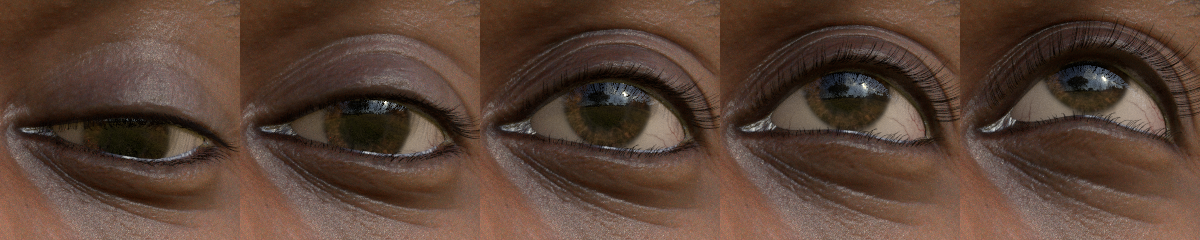
\includegraphics[width=\columnwidth]{eyelid_motion.png}
    \caption{Eyelids are posed by interpolating between blend shapes based on gaze direction. Note how we simulate the folding of the skin above and below the eye.}
    \label{fig:eyelids}
\end{figure}

% \commentY{At least we should give a different subsection title covering both eyelid motion and eyelashes?}
Eyelashes are short curved hairs that grow from the edges of the eyelids.
These can occlude parts of the eye and affect eye tracking algorithms, so are simulated as part of our comprehensive model.
We followed the approach of {\'S}wirski and Dodgson~\cite{swirski2014rendering}, and modelled eyelashes using directed hair particle effects.
Particles were generated from a control surface manually placed below the eyelids.
To make them curl, eyelash particles experienced a slight amount of gravity during growth (negative gravity for the upper eyelash).